% ★★ 中档
\newcommand{\qConicHardEllipseDotProductStem}{
已知椭圆 $C: \frac{x^2}{4} + \frac{y^2}{3} = 1$，点 $F(1, 0)$ 为右焦点．过点 $F$ 且斜率不为 $0$ 的直线 $l$ 与椭圆 $C$ 交于不同的两点 $A, B$．设坐标原点为 $O$，求 $\vec{OA} \cdot \vec{OB}$ 的取值范围．
}
\newcommand{\qConicHardEllipseDotProductFigure}{
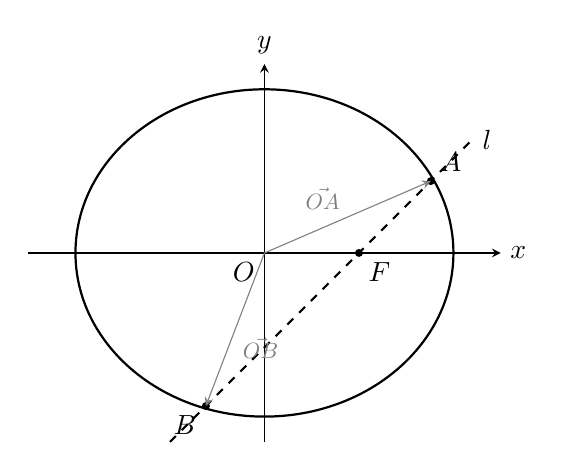
\begin{tikzpicture}[scale=1.2, >=stealth]
  % Axes
  \draw[->] (-2.5,0) -- (2.5,0) node[right] {$x$};
  \draw[->] (0,-2.0) -- (0,2.0) node[above] {$y$};
  \node[below left] at (0,0) {$O$};
  
  % Ellipse
  \draw[thick] (0,0) ellipse (2.0 and 1.732);
  
  % Focus F(1,0)
  \coordinate (F) at (1.0, 0);
  \fill (F) circle (1.2pt) node[below right] {$F$};
  
  % Line l: x = y + 1 => y = x - 1
  % Intersects x^2/4 + y^2/3 = 1 => 3x^2 + 4(x-1)^2 = 12 => 7x^2 - 8x - 8 = 0
  % roots: x1 = 1.76, y1 = 0.76; x2 = -0.62, y2 = -1.62
  \coordinate (A) at (1.76, 0.76);
  \coordinate (B) at (-0.62, -1.62);
  \fill (A) circle (1.2pt) node[above right] {$A$};
  \fill (B) circle (1.2pt) node[below left] {$B$};
  
  % Draw line and vectors
  \draw[thick, dashed] (-1.0, -2.0) -- (2.2, 1.2) node[right] {$l$};
  \draw[->, thin, gray] (0,0) -- (A) node[midway, above left, scale=0.8] {$\vec{OA}$};
  \draw[->, thin, gray] (0,0) -- (B) node[midway, below right, scale=0.8] {$\vec{OB}$};
\end{tikzpicture}
}
\newcommand{\qConicHardEllipseDotProductAnswer}{
$\vec{OA} \cdot \vec{OB}$ 的取值范围为 $[-4, -\frac{5}{4})$．
}
\newcommand{\qConicHardEllipseDotProductSolution}{
\begin{proof*}
因为过点 $F(1, 0)$ 且斜率不为 $0$ 的直线与椭圆交于不同的两点，
所以直线 $l$ 可设为：$x = ty + 1$ ($t \in \mathbb{R}$)，一般式为 $x - ty - 1 = 0$，对应硬解系数为 $A=1, B=-t, C=-1$．\\
椭圆 $C: \frac{x^2}{4} + \frac{y^2}{3} = 1$，对应参数 $a^2=4, b^2=3$．\\
此时统一分母为 $D = A^2a^2 + B^2b^2 = 1^2(4) + (-t)^2(3) = 3t^2 + 4$．\\
相交充要条件为 $D > C^2 \implies 3t^2+4 > 1$ 恒成立，判别式 $\Delta = 144(t^2 + 1) > 0$ 恒成立．\\
设 $A(x_1, y_1), B(x_2, y_2)$，联立消去 $x$ 得一元二次方程 $(3t^2+4)y^2 + 6ty - 9 = 0$，应用硬解定理直接写出纵坐标韦达公式：
\[
y_1 + y_2 = -\frac{2BCb^2}{D} = -\frac{6t}{3t^2 + 4},\qquad y_1y_2 = \frac{b^2(C^2-A^2a^2)}{D} = -\frac{9}{3t^2 + 4}
\]
同时，为了求数量积 $\vec{OA} \cdot \vec{OB} = x_1x_2 + y_1y_2$，我们直接写出横坐标之积 $x_1x_2$：
\[
x_1x_2 = \frac{a^2(C^2 - B^2b^2)}{D} = \frac{4[(-1)^2 - (-t)^2(3)]}{3t^2 + 4} = \frac{4 - 12t^2}{3t^2 + 4}
\]
利用此公式，可免去常规消元后对 $x_1x_2 = (ty_1+1)(ty_2+1)$ 的代数展开与化简，极大缩减了计算量．

因此，向量数量积：
\[
\vec{OA} \cdot \vec{OB} = x_1x_2 + y_1y_2 = \frac{4 - 12t^2}{3t^2 + 4} - \frac{9}{3t^2 + 4} = \frac{-12t^2 - 5}{3t^2 + 4}
\]
利用分离常数法化简分式：
\[
\vec{OA} \cdot \vec{OB} = \frac{-4(3t^2 + 4) + 11}{3t^2 + 4} = -4 + \frac{11}{3t^2 + 4}
\]
因为 $t \in \mathbb{R}$，所以 $t^2 \geq 0$，从而 $3t^2 + 4 \geq 4$．\\
因此可得：
\[
0 < \frac{11}{3t^2 + 4} \leq \frac{11}{4}
\]
两边同时减去 $4$ 得：
\[
-4 < -4 + \frac{11}{3t^2 + 4} \leq -\frac{5}{4}
\]
故 $\vec{OA} \cdot \vec{OB}$ 的取值范围为 $[-4, -\frac{5}{4})$．
\end{proof*}
}
\newcommand{\qConicHardEllipseDotProductDiagnosis}{
\errortag{横截式设法缺失} 部分学生习惯设直线为 $y = k(x-1)$，当直线斜率不存在（即垂直于 $x$ 轴）时，需要单独讨论，增加了书写和漏解的风险；此外，设 $y = k(x-1)$ 联立出的 $x$ 的二次方程在求数量积时需要将 $y_1y_2$ 用 $k^2(x_1-1)(x_2-1)$ 展开，计算极其冗长，容易出错．而采用 $x = ty + 1$ 的横截式可以直接通过 $y$ 的韦达定理进行极简计算．
}
